%==============================================================================
% Section 4: Boundary / interface response
%==============================================================================
\section{Boundary / Interface Response}
\label{sec:boundary}

This section addresses the second-layer boundary/cobordism response.  We
present the geometry-wise inventory, the observable taxonomy, the pairwise
cobordism dictionary, and the geometric scaffold layer as a single structure.
While the bulk layer is mainly concerned with ``what each geometry allows in
isolation,'' the second layer makes explicit ``what survives as an observable
on the boundary'' and ``which observables make geometry pairs comparable''.

\subsection{CZ Inflow and Notation}
\label{sec:boundary:cz}

In the second layer at least three different 3-forms must be carefully
distinguished:
\begin{itemize}
  \item $\Ctor$: torsion-CS 3-form,
  \item $\Csig$: spinor CS 3-form,
  \item $\Cadj$: adjoint CS 3-form.
\end{itemize}
We write the Chandia--Zanelli inflow \cite{Chandia1997} as
\begin{equation}
  \SCZ[M_3] = \frac{k_{\mathrm{cl}}}{4\pi^2}\int_{M_3} \Ctor.
\end{equation}
The relation
\begin{equation}
  \mathrm{NY} = \dd \Ctor,
  \qquad
  \dd \Ctor = T^a\wedge T_a + R_{ab}\wedge e^a\wedge e^b
\end{equation}
between the Nieh--Yan density and $\Ctor$ then connects the boundary inflow
directly to NY.  By contrast the APS spectral entry \cite{APS1975} is
defined via $\Csig = \Tr_\sigma(\omega\wedge \dd\omega + \tfrac{2}{3}\omega^3)$,
constructed only from the Levi--Civita connection; the two forms must not
be conflated.  The adjoint CS 3-form $\Cadj$ appears at intermediate stages
of the APS argument but is not the final spectral observable itself
(Appendix~\ref{app:E:E8}).

This distinction is essential for the taxonomy that follows.  The strict APS
entry of $\Nilthree$ and the frame-bundle-normalised torsional-charge entry
of $\Sthree$ are both parity-odd boundary quantities, but they belong to
different families.  Even within the spectral family, moreover, the source is
not uniform: the strict value of $\Nilthree$ is a local spectral core
provided by a non-zero Levi--Civita spinor CS integral, whereas the APS
branch on the compact $\Solthree$ benchmark is a global spectral branch
that arises from kernel/spin-structure data while the local CS integral
itself vanishes.

\subsection{Geometry-Wise Boundary Inventory}
\label{sec:boundary:inventory}

The geometry-wise boundary inventory is summarised as follows.

\begin{table}[H]
\centering
\resizebox{\linewidth}{!}{%
\begin{tabular}{lcccc}
\toprule
Entry & $\Tthree$ & $\Nilthree$ & $\Sthree$ & $\Solthree$ \\
\midrule
CS interface jump & absent & present & present & absent \\
APS $\eta$-invariant & $0$ & strict $+1/2$ (local) & $0$ & $0/1$ (Sol-A / Sol-P) \\
CZ inflow & absent & activated & activated & absent \\
edge / interface mode & minimal & activated & activated & spin-sensitive \\
boundary tag & trivial benchmark & APS local core & torsional-charge active & global spectral branch \\
\bottomrule
\end{tabular}%
}
\caption{Geometry-wise boundary inventory.}
\label{tab:boundary}
\end{table}

The principal entry of $\Nilthree$ is the strict APS spectral core, with
canonical value
\begin{equation}
  \etaAPS(\Nilthree) = +\frac{1}{2}.
\end{equation}
The Heisenberg mode decomposition shows that, with PPA spin structure, the
condition $p_2\in\mathbb{Z}+1/2$ excludes the $p_2 = 0$ zero mode, so that the
$n=0$ spin-up branch alone carries the spectral asymmetry.  The value itself
is obtained from the Levi--Civita spinor Chern--Simons integral of $\Nilthree$,
\begin{equation}
  \int_Y \Csig = -\frac{1}{2},
\end{equation}
combined with the DPPU orientation convention
$\etaAPS = -\int_Y \Csig$, giving
\begin{equation}
  \etaAPS = +\frac{1}{2}, \qquad \eta(0) = 2\etaAPS - h = 1
\end{equation}
(Appendix~\ref{app:E:E10}; verification: \texttt{paper04/eta\_aps\_nil3.py}).
Crucially, this spectral value originates from Levi--Civita spinor spectral
data rather than from the torsion-CS sector.  Although $\Nilthree$ also
carries CZ inflow, the strict core that takes precedence is the spectral
family, and its source is local.  As benchmarks, the PPA spin structure on
$\Tthree$ and the Levi--Civita Dirac on round $\Sthree$ both have spectra
exactly symmetric under $\lambda\leftrightarrow -\lambda$, giving
$\etaAPS = 0$ (verification: \texttt{proofs/aps\_zero\_t3\_s3.py}).

\begin{figure}[H]
\centering
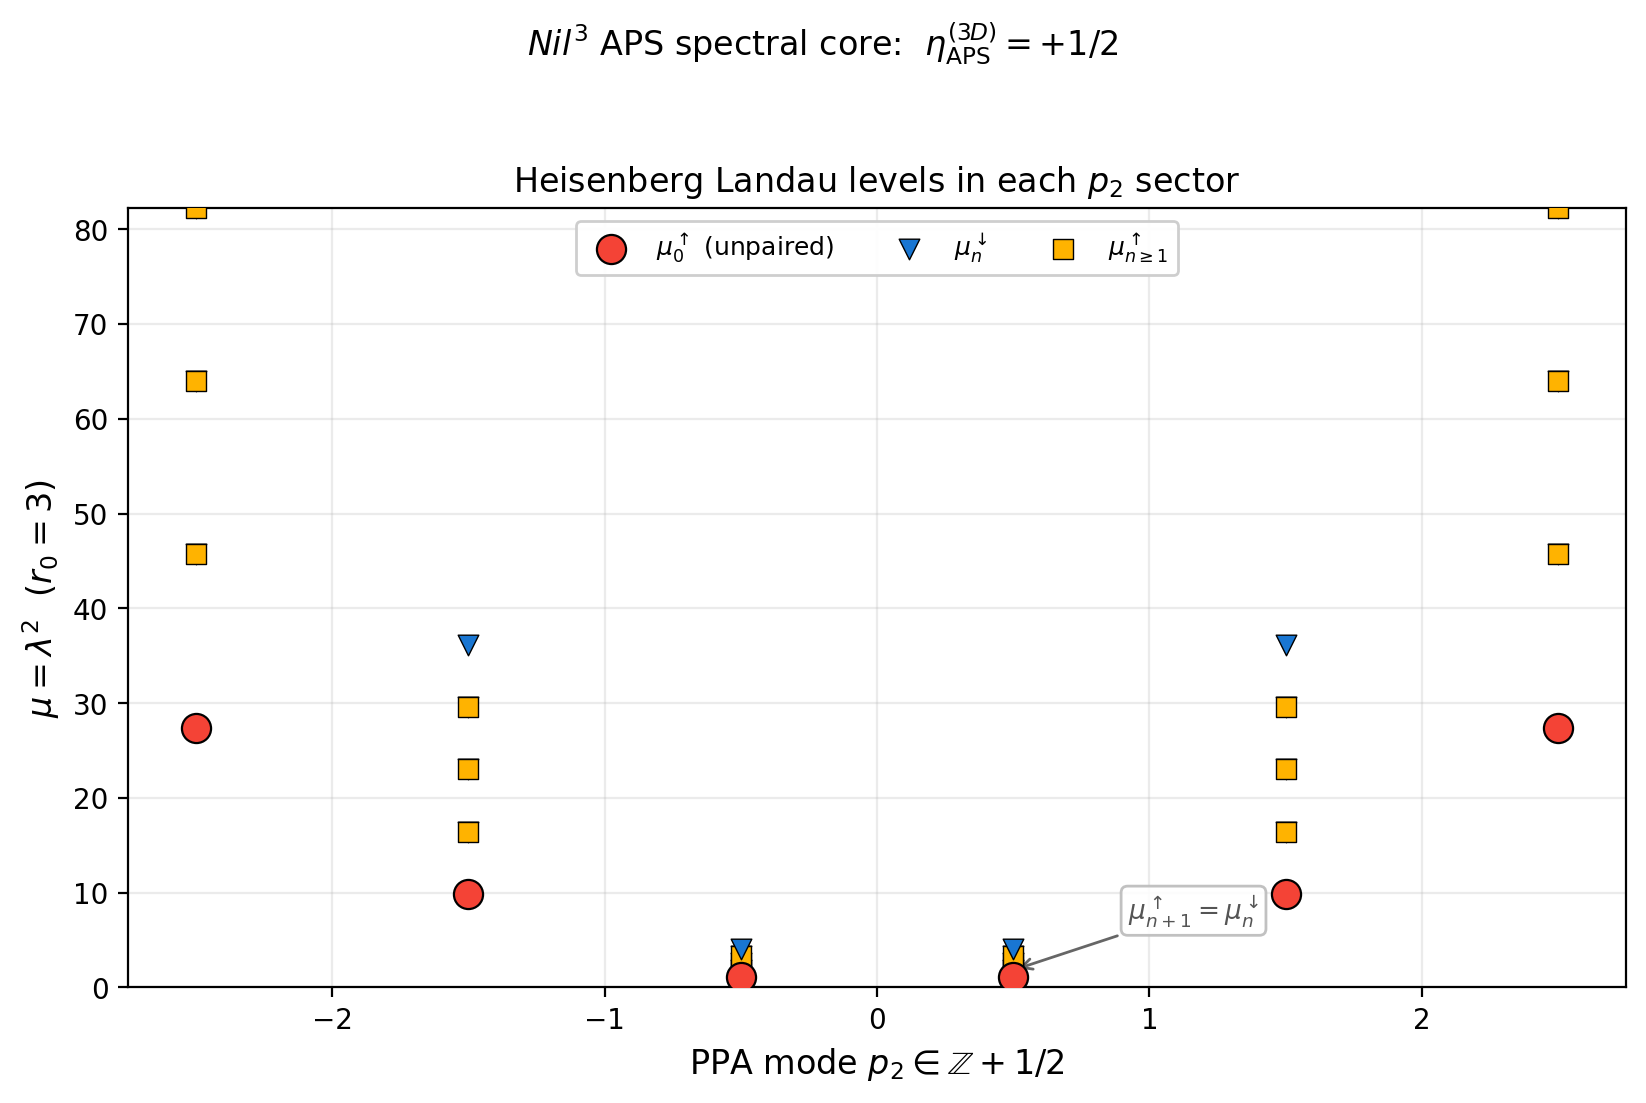
\includegraphics[width=0.85\linewidth]{figures/fig04_nil3_aps.png}
\caption{$\Nilthree$ Heisenberg Landau-level spectrum and the construction of
$\etaAPS$.  Under the PPA spin structure the $n=0$ spin-up branch carries
the spectral asymmetry, and the Levi--Civita spinor CS integral gives
$\etaAPS(\Nilthree) = +1/2$.}
\label{fig:nil3_aps}
\end{figure}

For $\Solthree$ the situation is different.  Taking the compact mapping-torus
benchmark
\begin{equation}
  M_A = T^2\rtimes_A \Sone,
  \qquad
  A = \begin{pmatrix}2 & 1 \\ 1 & 1\end{pmatrix},
\end{equation}
together with the two spin structures Sol-P and Sol-A tracked within DPPU,
the local Levi--Civita Chern--Simons integral itself vanishes:
\begin{equation}
  \int_Y \Csig = 0.
\end{equation}
Here ``Sol-P'' denotes the benchmark with periodic base circle and periodic
fibre, and ``Sol-A'' the benchmark with anti-periodic base circle and
periodic fibre.  The Dirac kernel branches as
\begin{equation}
  h(\text{Sol-P}) = 2, \qquad h(\text{Sol-A}) = 0,
\end{equation}
and the antilinear time-reversal symmetry gives $\eta(0) = 0$, so that
\begin{equation}
  \etaAPS(\text{Sol-P}) = 1, \qquad
  \etaAPS(\text{Sol-A}) = 0
\end{equation}
(Appendix~\ref{app:E:E10b}; verification: \texttt{proofs/eta\_aps\_sol3.py}).
$\Solthree$ is therefore not a ``local APS core'' but a global spectral
branch that switches on/off according to the compact quotient and the spin
structure.

\begin{figure}[H]
\centering
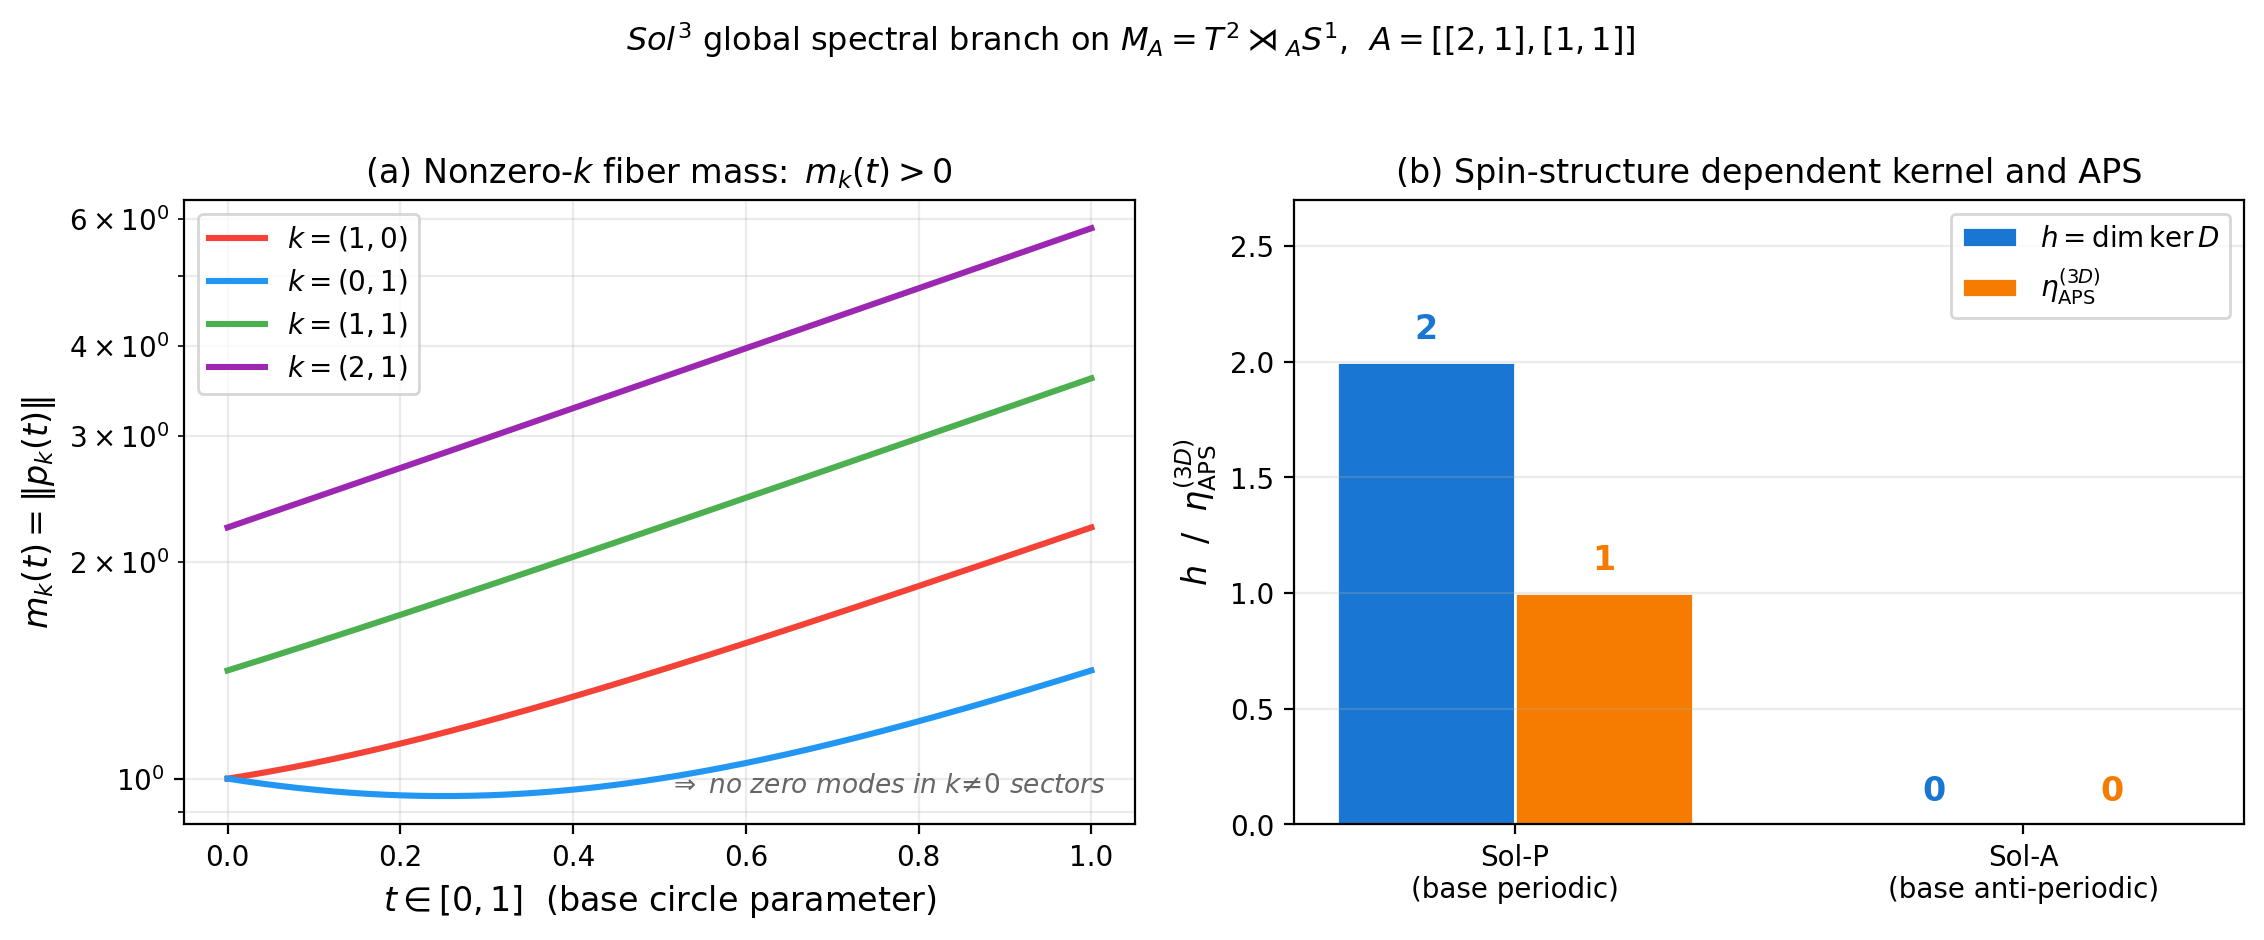
\includegraphics[width=0.85\linewidth]{figures/fig05_sol3_global_spectral.png}
\caption{Global spectral branch of $\Solthree$.  On the compact mapping-torus
benchmark the kernel dimension $h$ and $\etaAPS$ branch between Sol-P and
Sol-A; the on/off switching is driven by global / spin-structure data
rather than by the local CS integral.}
\label{fig:sol3_global}
\end{figure}

The principal entry of $\Sthree$ is the frame-bundle-normalised
torsional-charge core characterised by
\begin{equation}
  \Ntop = 6 r_0^2.
\end{equation}
The geometric part follows from the structure constants
$C^i{}_{jk} = (4/r_0)\,\epsilon^i{}_{jk}$ via
$T^i = \tfrac{1}{2}C^i{}_{jk}\,e^j\wedge e^k$ and
\begin{equation}
  \Ctor = e_i\wedge T^i = \frac{12}{r_0}\,\mathrm{vol}_{\Sthree}
  \quad\Longrightarrow\quad
  \int_{\Sthree}\Ctor = 24\pi^2 r_0^2.
\end{equation}
The factor $1/(4\pi^2)$ is the frame-bundle normalisation associated with
$\pi_3(SO(3)) = \mathbb{Z}$ ($T_R = 1$), leading to $\Ntop = 6 r_0^2$
(Appendix~\ref{app:E:E9}).  Since no extra quantisation condition on $r_0$
is imposed, $\Ntop$ here is the frame-bundle-normalised torsional charge.
The interface CS jump and the CZ inflow belong to this torsional sector and
underpin the role of $\Sthree$ in the pairwise dictionary as the
torsional-charge-led geometry.

$\Tthree$ has all boundary entries trivial and serves as a benchmark.  Yet
$\Solthree$ is CS-inert while still carrying an EC slice minimum and a rigid
scaffold; in the boundary layer it can support a global spectral branch
depending on the compact quotient and the spin structure.  Collapsing
$\Tthree$ and $\Solthree$ into a single second-layer class is therefore
inaccurate.  Independently of the presence/absence of a boundary spectral
branch, the fact that $\Solthree$ has a distinct, non-flat background
geometry is preserved.

\subsection{Observable Taxonomy}
\label{sec:boundary:taxonomy}

We classify the second-layer observables into the following three families.

\begin{table}[H]
\centering
\resizebox{\linewidth}{!}{%
\begin{tabular}{llllc}
\toprule
Family & Representative & Carrier & Value type & Canonical geometry \\
\midrule
spectral & $\etaAPS$ & LC spectral data ($\Csig$ and/or kernel/spin) & half-int. / int.\ branch & $\Nilthree$ (local), $\Solthree$ (global) \\
torsional-charge & $\Ntop$ & frame-bundle normalisation of $\Ctor$ & frame-bundle-norm.\ torsional charge & $\Sthree$ \\
inflow & $\SCZ$ & $\Ctor$ & boundary functional & $\Nilthree$, $\Sthree$ \\
\bottomrule
\end{tabular}%
}
\caption{Three observable families of the second layer.}
\label{tab:taxonomy}
\end{table}

These three families furnish the observable taxonomy of the second layer.
The crucial point is that, although $\etaAPS$ and $\Ntop$ are both
non-trivial boundary quantities, they are not of the same type and should
not be subtracted directly.  Quantities universally comparable in pairwise
comparison reside instead on the side of the inflow functional written in
terms of $\Ctor$.

\subsection{Pairwise Cobordism Dictionary}
\label{sec:boundary:pairwise}

Six pairs are obtained from the four geometries.  We summarise the dominant
observable and source relation for each pair.

\begin{table}[H]
\centering
\resizebox{\linewidth}{!}{%
\begin{tabular}{lcll}
\toprule
Pair & Class & Dominant observable & Note \\
\midrule
$\Sthree \leftrightarrow \Tthree$ & torsional / trivial & frame-bundle-norm.\ torsional charge & $\Sthree$ benchmark \\
$\Sthree \leftrightarrow \Nilthree$ & torsional / local spectral & mixed & torsional-charge crosses local spectral \\
$\Sthree \leftrightarrow \Solthree$ & torsional / global spectral & spin-sensitive & torsional-led for Sol-A; mixed for Sol-P \\
$\Tthree \leftrightarrow \Nilthree$ & trivial / local spectral & spectral & $\Nilthree$ local core dominates \\
$\Tthree \leftrightarrow \Solthree$ & trivial / global spectral & spin-sensitive & Sol-A: trivial; Sol-P: global spectral \\
$\Nilthree \leftrightarrow \Solthree$ & local / global spectral & spectral & source comparison within spectral family \\
\bottomrule
\end{tabular}%
}
\caption{Pairwise cobordism dictionary.}
\label{tab:pairwise}
\end{table}

\begin{figure}[H]
\centering
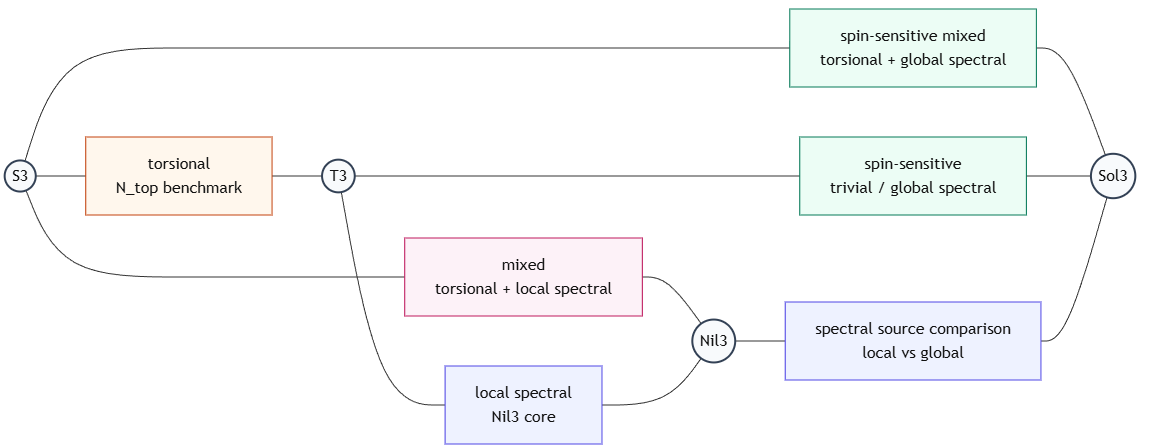
\includegraphics[width=0.9\linewidth]{figures/fig06_pairwise_cobordism_dictionary.png}
\caption{Pairwise cobordism dictionary.  The four geometries form the
vertices of a pair graph; the six pairs are labelled with the dominant
observable and the spin-sensitivity.  Pairs containing $\Sthree$ tend to be
torsional-charge-led, whereas pairs containing $\Solthree$ admit a global
spectral branch governed by the compact quotient and the spin structure.}
\label{fig:pairwise}
\end{figure}

This table captures the comparison logic of the paper most directly: the
geometry-wise inventory translated into the language of pairwise cobordism.
In particular, $\Sthree\leftrightarrow\Nilthree$ is the intersection of the
torsional-charge family and the local spectral family, while
$\Nilthree\leftrightarrow\Solthree$ encodes a ``local vs.\ global'' source
distinction within the spectral family itself.  $\Tthree\leftrightarrow\Solthree$
is not a uniformly inert pair either: it overlaps the trivial benchmark for
Sol-A, while a global spectral branch arises for Sol-P, making it a
spin-sensitive pair.

The advantage of the pairwise dictionary is that it makes simultaneously
explicit ``which observable family is the subject of comparison'' and
``whether the value is local or global''---features hard to read off from a
geometry-by-geometry inventory alone.  The tendency that pairs containing
$\Sthree$ are torsional-charge-led, those containing $\Nilthree$ are
local-spectral-led, and those containing $\Solthree$ may carry a global
spectral branch depending on the compact quotient and spin structure
underpins the concise statement of the selection rules.

\subsection{Geometric Scaffold Layer}
\label{sec:boundary:scaffold}

While not an observable family, we also record the following scaffold-layer
quantities, which characterise the background geometry.

\begin{table}[H]
\centering
\begin{tabular}{lccc}
\toprule
Geometry & $C^2_\LC$ & spin-2 rigidity tag & $\AKK / K^2$ \\
\midrule
$\Tthree$ & $0$ & trivial & $0$ \\
$\Nilthree$ & $4/(3R^4)$ & non-rigid & $2/3$ \\
$\Sthree$ & $0$ & non-rigid & $0$ \\
$\Solthree$ & $16/(3R^4)$ & rigid & $2/3$ \\
\bottomrule
\end{tabular}
\caption{Geometric scaffold quantities.}
\label{tab:scaffold}
\end{table}

\begin{figure}[H]
\centering
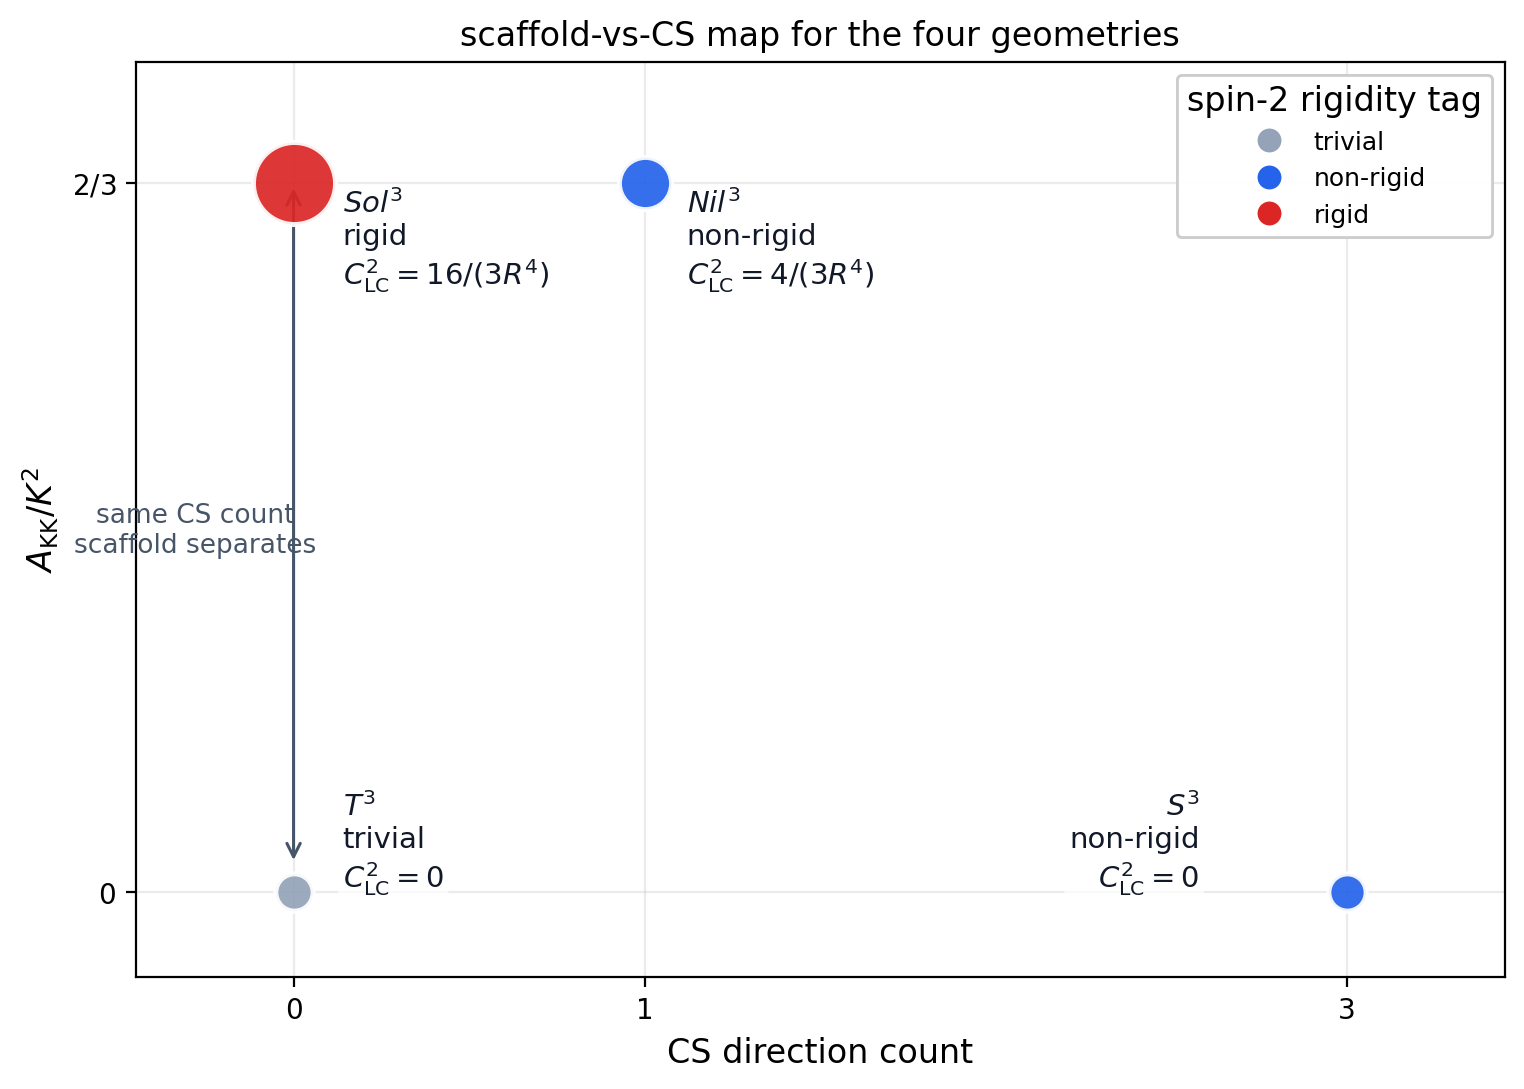
\includegraphics[width=0.85\linewidth]{figures/fig07_scaffold_vs_cs.png}
\caption{Scaffold-vs-CS scatter.  The horizontal axis is the CS direction
count, the vertical axis is $\AKK/K^2$, the marker size encodes
$C^2_\LC$, and the colour encodes the spin-2 rigidity tag.  $\Tthree$ and
$\Solthree$ share CS count $0$ but separate in the scaffold layer.}
\label{fig:scaffold}
\end{figure}

The spin-2 rigidity tag is not a strict numerical invariant but a
scaffold label summarising the zero pattern of the squash/shear Hessian.
``Rigid'' refers to the $\Solthree$ frame rigidity
\begin{equation}
  \frac{\partial^2 V}{\partial \varepsilon^2}
  = \frac{\partial^2 V}{\partial s^2}
  = \frac{\partial^2 V}{\partial \varepsilon\, \partial s} = 0,
\end{equation}
``trivial'' to the flat kinematic zero of $\Tthree$, and ``non-rigid'' to the
non-zero spin-2 Hessian of $\Nilthree$ / $\Sthree$.

This Hessian zero pattern is a non-trivial consequence of the fact that the
volume-preserving deformation
$f_1=(1+\varepsilon)^{2/3}(1+s),\ f_2=(1+\varepsilon)^{-2/3}/(1+s)$
of $\Solthree$ leaves the structure constants independent of $\varepsilon, s$
(Appendix~\ref{app:E:E1}); the script \texttt{proofs/sol3\_structure.py}
verifies that the three second derivatives vanish directly.

The KK anisotropy is defined as
\begin{equation}
  \AKK := \sum_{i=0}^{2}(m_i^2-\bar m^2)^2,
  \qquad
  \bar m^2 := \frac{1}{3}\sum_{i=0}^{2} m_i^2,
\end{equation}
normalised by $K^2 := \KMxw^2$; we record
$\AKK/K^2 = 0,\,2/3,\,0,\,2/3$ as the scaffold datum.

The role of this layer is not to add a new observable family but to explain
``why the activation pattern of the three families differs across the
geometries''.  Both $\Tthree$ and $\Solthree$ lack a local CS core, yet they
are separated in the bulk layer by the presence/absence of an EC slice
minimum and a rigid scaffold, and they are further distinguished in the
boundary layer by the global spectral branch dependent on the compact
quotient and spin structure.  On the Sol-A benchmark a trivial spectral
profile coincident with $\Tthree$ appears, whereas the Sol-P benchmark
raises a global spectral branch with $\etaAPS = 1$.  The geometric
distinction---that $\Tthree$ is flat and inert while $\Solthree$ carries a
non-vanishing Weyl curvature, an EC slice minimum, a biaxial KK splitting,
and frame rigidity---persists nonetheless.  This distinction does not
amount to introducing further observable families, but it is indispensable
for a complete characterisation of the geometries.

The second-layer dictionary thus closes through the three views:
geometry-wise, pairwise, and scaffold.  In the next section we combine these
with the bulk layer and compress the contents into selection rules instead of
an enumeration of individual computations.
